% !TeX spellcheck = en_US
% !TeX encoding = UTF-8
% !TeX root = ../thesis.tex

\chapter{Fundamentals}
This chapter introduces basic concepts used throughout this thesis.
First we discuss the basics of reinforcement learning and
the problem of robot learning.
Next we give an overview of policy search,
a sub-field of reinforcement learning,
as one method to solve the robot learning problem.
The Kullback-Leibler divergence (KL) is
introduced as an important information theoretic
measure of similarity metric between probability
distributions \citep{kullback1951information}.
Having discussed the underlying basics we can then
introduce the MORE algorithm \citep{abdolmaleki2015model}.
Finally, we will look at filtering from a Bayesian Estimation viewpoint and
review the Kalman filter for parameter estimation.

\section{Reinforcement Learning}
Reinforcement Learning (RL) is a subfield of Machine Learning concerned with agents
learning to interact with their environment, enabling them to solve tasks.
This is done through exploration and trial-and-error, trying to discover
cause and effect relationship between actions.
Compared to supervised learning and unsupervised learning it
more closely resembles the way humans learn. \\
As \citet{sutton2018reinforcement} puts it,
the term reinforcement learning relates to a class of problems,
solution methods and the field that studies these problems and solutions.
Some famous examples include playing games like Go
\citep{silver2016mastering} and Atari games \citep{mnih2013playing}.
Generally, RL is applicable to a large range of problems.
Whereas in supervised learning the best action is presented to the system,
the agent in a reinforcement learning setting receives a
reward (or punishment) for each action.
To gain information about the rewards the agent needs
to explore previously unused actions.
Dare to try new things or keep performing safe
well-known actions, this is the \textit{exploration-exploitation tradeoff}.
The agent should exploit actions he knows that
give decent reward, but he first
has to try different things to learn about these actions,
and then he has to progressively focus in on them.
The reward signal is typically a single scalar value, hence the amount of information
the agent receives is minimal compared to
supervised and unsupervised learning approaches.

The classical approach to formalizing problems in RL is through
Markov Decision Processes (MDPs).
MDPs are a mathematical
framework for decision making in deterministic and stochastic environments.
MDPs focus on only three aspects
- sensation, action and goal, which are central
for reinforcement learning problems.
MDPs satisfy the Markov property, which
states that ``the future is independent
of the past given the present''. In our case this means
the next state $s'$ and the reward
only depend on the previous state $s$ and
action $a$ \citep{sutton1992reinforcement}.
An MDP can be formally defined as a tuple $(S, A, P, r)$:

\begin{itemize}
\item a set of states $s \in S$ that describe the environment,
\item a set of actions $a \in A$ that can be performed by the agent in
  the environment
\item a transition function $P(s_{t+1} | s_t, a_t)$ that
  gives the probability of a new,
  state $s_{t+1}$ after an action $a_t$ has been taken in state $s_t$,
\item and a reward function $r(s_t, a_t)$ that specifies
  the immediate reward after taking action
  $a_t$ in state $s_t$.
\end{itemize}

The Markov property can be expressed as
$$ P(s_{t+1} | s_t, a_t, s_{t-1}, a_{t-1}\cdots) = P(s_{t+1} | s_t, a_t). $$
This recapitulates the notion of state - a state is a sufficient statistic
for predicting the future, rendering previous observations irrelevant.
In robotics, we may only find some approximate notion of state.

For our setting, we model the agent and its environment as a state $s \in S$.
The agent may perform action $ a \in A$ which can be
either discrete or continuous.
For every action step, the agent receives a reward $R$,
which is a scalar value.
The overarching goal is to find a mapping from states to actions,
called policy $\pi$, that picks actions in a way that
the reward is maximized.
We can distinguish an \textit{episodic} setting
from an on-going task.
In the episodic setting
the task is restarted after
the end of an episode and the goal is
to maximize the total reward per episode.
In on-going tasks the goal
is to simply achieve high average reward over
the whole life-time or one can use a formulation
with a discounted return (weighting the
future and past differently).

Generally, the goal is to find an optimal policy $\pi^*$,
a mapping from states to actions that
maximizes the expected return $J$.
Optimal behavior can be modeled in
different ways, resulting in different
definitions for expected return:
\begin{itemize}
\item for a finite-horizon model with horizon $H$ we get
$$ J = E \left\{\sum^H_{t=0} R_t \right\}, $$

\item a discounted reward can be modeled with
  a discount factor $\gamma$ (with $0 \leq \gamma < 1)$, which yields
$$ J = E \left\{\sum^{\infty}_{t=0} \gamma^{\; t} R_t \right\}. $$
\end{itemize}

Reinforcement learning can also be seen as
general case of optimal control as in \citet{sutton1992reinforcement}.
While optimal control assumes perfect knowledge, RL uses approximations
and data-driven techniques.

%TODO: - write about Value learning, and shortly name traditional methods (multiarmbandit,
%DP, Temporal difference learning)


\section{Robot Learning}
The sub-field where reinforcement learning and machine learning
intersect with robotics is called \textit{Robot Learning}. It aims to bridge
the gap between programmed robots,
with fine tuned controllers  and fully autonomous robots.
As proposed in \citet{deisenroth2013survey}, robot control can be modeled as
a reinforcement learning problem. \\
The state space $\mathbf{x}$ in robotic tasks is high dimensional and
made up of
the internal state of the robot (e.g., joint position, body position,
camera images)
and external state (e.g. object locations, lighting). The true state is
not observable and also not noise free. 
The robot chooses its next motor control $u$ according to a policy $\pi$.
This policy $\pi$ may
be deterministic $u = \pi(s)$ or stochastic $u \sim \pi(s,a) = P(u | s)$.
The motor commands $u$ alter the state according to the probabilistic
transition function $p(\mathbf{x}_{t+1} | x_t, u_t)$. This transition function
is not known, in model-based policy search this function is learned from data and
used to improve the policy.
Collectively the states and actions of the robot form a
\textit{trajectory} $\tau = (x_0, u_0, x_1, u_1,...)$ which is also called
a \textit{rollout} or a \textit{path}.
There has to be a numeric scoring system assessing the quality
of the robots trajectory and returning a reward signal $R(\tau)$.
For \textit{episodic learning tasks} the task ends after a given number $T$ of time
steps. Then the accumulated reward $R(\tau)$ for a trajectory is given by

$$ R(\tau) = r_T(x_T) + \sum^{T-1}_{t=0} r_t(x_t,u_t) $$

where $r_t$ is an instantaneous reward function (e.g. a punishment for energy consumed)
and $r_T$ the final reward, when performing a reaching task this may take the
form of a quadratic punishment term for deviation from the goal posture.

If we consider an infinite-horizon for an on-going task we get
$$ R(\tau) = \sum^{\infty}_{t=0} \gamma^{\; t} r(x_t, u_t) $$
where $\gamma \in [0,1)$ is a discount factor that discounts rewards further in the future.

Many tasks in robotics can thus be formulated as choosing an optimal control
policy $\pi^*$ that maximizes the expected accumulated reward

$$ J_{\pi} = \mathbb{E}[R(\tau) | \pi] = \int R(\tau) p_{\pi}(\tau) d\tau $$
where $R(\tau)$ defines the objectives of the task, and $p_{\pi}(\tau)$ is the
distribution over trajectories $\tau$.

Formulating robotic tasks in this way allows us to use methods from
reinforcement learning. 

\subsection{Challenges}
Reinforcement learning is in general a difficult problem. One reason
for this is that the reward signal may be given only occasionally and
even then it may be unclear which of
the agents actions were responsible for a certain
reward signal. 

Robotics is different compared to other fields where Reinforcement Learning
is used extensively. First of all the states and actions of the robots in the
real world are inherently continuous requiring us to
deal with the resolution.
In addition the state space can have a high dimensionality and
working with real world systems on real hardware is costly and
makes manual interventions necessary.
Robots require algorithms to run in real-time and working with
real sensors further introduces discrepancy between sensing and
execution.

Most traditional methods from RL like
TD-learning \citep{sutton2018reinforcement}
have been unfit for these particular requirements of robotic tasks.
Stressing the importance of robotics as a testing ground for RL that
demands new developments and innovative research.
We will now discuss some problems encountered when applying
RL to robotics, this treatment does only focus on a certain
set of challenges and is not exhaustive.

\subsubsection{Curse of Dimensionality}
The term ``Curse of Dimensionality'' was coined by \citet{Bellman:1957} when
he explored optimal control in higher dimensions and encountered
an exponential explosion of the states and actions.
For example, for the evaluation of our algorithm we run a simulation of a
simple planar reaching task
with a 5 link robot arm using Dynamic Movement Primitives \citep{ijspeert2002learning}
for policy representation and get a 25 dimensional state.
Especially modern anthropomorphic robots tend to have many degrees of
freedom.

The agent in RL generally needs to collect data throughout the entire
state-space to ensure global optimization, for robotics dealing with
three dimensional space makes this very difficult.
To alleviate this problem  a widespread idea is to use expert demonstration
to get a good initialization for the agent's policy. This
eliminates the need to explore the entire search space, instead the
agent can focus on locally optimizing the initial policy.
This concept of imitation learning focuses on the problem of ``learning
from demonstrations'' which plays an important role
for robotics \citep{Osaetal18}. Imitation learning
will enable domain experts to teach motions and
skills without special knowledge about robotics, which will be crucial
when robots start making their way from factories into everyday life.

\subsubsection{Curse of Real-world Samples}
Robot hardware is expensive and suffers from wear and tear, making
costly maintenance necessary. Hence, safe methods for real robots
should avoid big jumps in policy updates, as such sudden changes may
result in unpredictable movements and consequently damage the robot.
This problem is commonly referred to as \textit{safe exploration}.
Whereas in traditional reinforcement learning
safe exploration does not receive much attention,
it has become a key issue for robot learning \citep{schneider1997exploiting}.
Different external factors like temperature may change the robot dynamics and
additional uncertainty from the sensors makes it difficult to reproduce and
compare results.

Most tasks also require a ``human in the loop'' who either supervises the robot
or resets the setup after one episode. Even if this can be avoided the learning
speed simply cannot be sped up.
For a single robot the training time has a natural limit
and in total only relatively few executions can be completed.
One method for gathering more data is ``collective robot learning'' described in
\citet{kehoe2015survey}. The idea is for multiple robots to
share their data on trajectories, policies and outcomes. Currently this seems only
viable for large corporations with significant capital.
Thus, in robot learning the constraint of using only a small number of trials
is given more weight than limiting memory consumption or computational complexity.
Stressing the importance of developing sample efficient algorithms.
Generally the state represented by sensors slightly lags behind the real
state due to processing and communication delays. This is in stark contrast to
most other reinforcement learning algorithms, which assume actions to take effect
instantaneously.

\subsubsection{Curse of Goal Specification}
Defining a good reward function in robot reinforcement learning is
difficult and often needs a lot of domain knowledge and expertise.
There are certain trade-offs to keep in mind, for example performing
a powerful swing for a hitting task may yield high reward but may damage
or shorten the life-time of the robot.
Reinforcement Learning algorithms may solve tasks
in unintended ways exploiting the reward function in an unforeseen style
\citep{ng1999policy}.

Inverse reinforcement learning \citep{russell1998learning}
provides an alternative  to specifying the reward function manually.
The goal of inverse reinforcement learning is to recover the unknown
reward function from the expert's trajectories.

Still, learning algorithms are rarely employed on robots
for real daily usage. Also most
algorithms are over fitted to a particular robot architecture
and do not generalize to other robots easily.
Even minor flaws or errors in the employed method can completely prevent
success of learning.
Nonetheless, appropriately chosen algorithms and rewards functions
can already achieve promising results, but as 
a large number of different methods exist 
there is no clear recipe for robot learning.
Stressing that robot learning still has a lot of open problems,
and will continue to grow as a research field.

\subsection{Policy Search}
Many traditional methods in RL try to estimate the
expected long-term reward of a policy for each state $\mathbf{x}$
and time step $t$, which leads to formulation of the value function $V^{\pi}_t(\mathbf{x})$.
With the value function we can asses the quality of executing action
$\mathbf{u}$ in state $\mathbf{x}$. This assessment is used
to directly compute the policy by action selection or to update
the policy $\pi$. As value function methods typically require
to fill the complete action-space they struggle with
the high dimensionality encountered in robotics.
Thus policy search methods have become more common
for applying RL to robotics.
Policy search methods opposed to value-based methods
use parameterized policies $\pi_{\theta}$ and search
directly in the parameter space $\Theta$. This allows using RL with
high-dimensional continuous action spaces encountered
in robotics by reducing the search space of possible policies.
Policy search further allows the usage of predefined
task-appropriate policy representations like Dynamic
Movement Primitives \citep{schaal2005learning}, as well
as easily integrating imitation learning
for policy initialization.

Generally, we can divide policy search into model-free and model-based and
differentiate whether stochastic or deterministic trajectories are used.
Model-free policy search uses trajectories from the robot directly
for updating the policy. Model-based methods use the data
from the robot to learn a model of the robot. This model is then used
to generate trajectories that are used for policy updates.
Due to their simplicity and by avoiding the need of learning a model,
which further introduces the problem of under-modeling,
model-free methods have been widely employed.

The most important concept is computing the policy updates.
Both model-free and model-based policy search use policy gradients (PG),
expectation-maximization (EM)-based updates, or
information-theoretic insights (Inf.Th.).

- For model-free algorithm the REINFORCE

- markov chain based Expectation maximzation (MC-EM)

- Inf. Theoretic REPS and MORE

\Cref{fig:policy}
gives an overview of the different policy search methods
and some example algorithms.


\begin{figure}[ht!]
  \centering
  \scalebox{0.9}{
\usetikzlibrary {backgrounds,fit}
    \begin{tikzpicture}
      \draw (1, 0.5) node [draw=black, rounded corners] (data) {Policy Search};

      \draw (-2.4, -1) node [fill=blue!80!black!30, rounded corners](model_free) {Model-free};
      \draw [-] (data) -- (model_free);      
      \draw (-2.4, -2) node [fill=red!80!black!30, rounded corners](free) {Stoch. Traj.};
      \draw [-] (model_free) -- (free);      
      \draw (-3.5, -3) node [fill=green!80!black!20, rounded corners](free_pg) {PG};
      \draw (-2.5, -3) node [fill=green!80!black!20, rounded corners](free_em) {EM};
      \draw (-1.25, -3) node [fill=green!80!black!20, rounded corners](free_inf) {Inf. Th.};
      \draw [-] (free) -- (free_pg);
      \draw [-] (free) -- (free_em);
      \draw [-] (free) -- (free_inf);
      
      
      \draw (4, -1) node [fill=blue!80!black!30, rounded corners] (model) {Model-based};
      \draw [-] (data) -- (model);
      
      \draw (2.25, -2) node [fill=red!80!black!30, rounded corners] (model_stoch) {Stoch. Traj.};
      \draw [-] (model) -- (model_stoch);      
      \draw (1.25, -3) node [fill=green!80!black!20, rounded corners](stoch_pg) {PG};
      \draw (2.25, -3) node [fill=green!80!black!20, rounded corners](stoch_em) {EM};
      \draw (3.5, -3) node [fill=green!80!black!20, rounded corners](stoch_inf) {Inf. Th.};
      \draw [-] (model_stoch) -- (stoch_pg);
      \draw [-] (model_stoch) -- (stoch_em);
      \draw [-] (model_stoch) -- (stoch_inf);

      
      \draw (6, -2) node [fill=red!80!black!30, rounded corners] (model_det) {Det. Traj.};
      \draw [-] (model) -- (model_det);      
      \draw (5, -3) node [fill=green!80!black!20, rounded corners](det_pg) {PG};
      \draw (6, -3) node [fill=green!80!black!20, rounded corners](det_em) {EM};
      \draw (7.25, -3) node [fill=green!80!black!20, rounded corners](det_inf) {Inf. Th.};
      \draw [-] (model_det) -- (det_pg);
      \draw [-] (model_det) -- (det_em);
      \draw [-] (model_det) -- (det_inf);

      %%%%%%%%%%%%%%%%%%%%%%%%%%%%%%%%%%%%%%%%%%%%%%%%%%%%%%%%%%%%%%
      % Examples
      %%%%%%%%%%%%%%%%%%%%%%%%%%%%%%%%%%%%%%%%%%%%%%%%%%%%%%%%%%%%%%
      \draw (-4.75, -5) node (examples) {\small \textbf{Examples:}};      
      \draw (-3.25, -5.6) node (reinforce) {REINFORCE};
      \draw (-1.25, -5.2) node (power) {PoWER};
      \draw (0.6, -5.4) node (reps) {REPS};
      \draw (2.2, -5.1) node (more) {MORE};      
      \draw [thick, dotted] (free_pg) to[out=-90,in=90] (reinforce);
      \draw [thick, dotted] (free_em) to[out=-90,in=90] (power);
      \draw [thick, dotted] (free_inf) to[out=-90,in=90] (reps);
      \draw [thick, dotted] (free_inf) to[out=-75,in=90] (more);      

      
      % \draw (4, -5.75) node (pegasus) {PEGASUS};
      \draw (5.5, -5) node (pilco)
      {$~~~~~~~~\quad\quad\quad\quad\quad$ PILCO $~~~~~~~\quad\quad\quad\quad\quad$};
      \draw [thick, dotted] (det_pg) to[out=-90,in=90] (pilco);

      \begin{scope}[on background layer]
        \node [thick, dashed, draw=black, rounded corners, fill=black!5,fit=
        (model_free) (free) (free_pg) (free_em) (free_inf)]{};
      \end{scope}
      
      \begin{scope}[on background layer]
        \node [thick, dashed, draw=black, rounded corners, fill=black!5,fit=
        (model) (model_det) (model_stoch)
        (det_pg) (det_em) (det_inf)
        (stoch_pg) (stoch_em) (stoch_inf)]{};
      \end{scope}
      
      \begin{scope}[on background layer]
        \node [thick, draw=black,fit=
        (examples)
        (reinforce) (power)
        (reps) (pilco)]{};
      \end{scope}
    \end{tikzpicture}
}
    \caption{\small
      Categorization of policy search into model-free policy
      search and model-based policy search.
      In stochastic trajectory generation 
      trajectories are directly sampled from the robot or
      in the model-based case from the learned model of the robot.
      Some Model-based methods also use deterministic trajectory prediction 
      and analytically predict the trajectory distribution
      instead of sampling from the system. Drawing based on
      \citet{deisenroth2013survey}
    }
    \label{fig:policy}
\end{figure}

% - TODO: include figure for policy search taxonomy
% (recreated from \citet{deisenroth2013survey})
% also include examples for each type (REINFORCE, REPS, PILCO,...)


In this thesis, we will focus on model free policy search methods
where the trajectories are generated by ``sampling'' from
the robot.
More specifically we will focus on stochastic
search algorithms, which are general black-box optimizers.
They are used in a wide range of fields like operations research,
machine learning and also policy search.
Since these algorithms do not use any knowledge about the
objective function it is straightforward to
apply them to policy search in the episode-based formulation.

Using stochastic search algorithms we keep an upper-level policy
$\pi_{\omega}(\theta)$ which selects the parameters of the
actual control policy $\pi_{\theta}(\mathbf{u} | \mathbf{x})$ of the robot.
Instead of directly finding the parameters $\theta$ of the
lower-level policy we want to find the parameter vector $\omega$ which
defines a search distribution over $\theta$. We can then use this
search distribution to directly explore the parameter space.


\section{Kullback-Leibler (KL) Divergence}
Several algorithms used for policy search like
NES \citep{wierstra2014natural} and REPS \citep{peters2010relative}
rely on the Kullback-Leibler divergence, also
known as the relative entropy, for controlling
the difference between the old and updated policy.
Working with real robots additionally requires to perform safe exploration. Big
exploration steps may result in damaging the hardware.
Specifically, it measures the Shannon entropy of one distribution relative to the
other. The KL divergence from $q$ to $p$ is defined as
$$ KL(p || q) = \int p(\theta) \text{ log} \left(\frac{p(\theta)}{q(\theta)}\right)
d \theta $$
where $p$ and $q$ are continuous probability distributions.
Note, that in general the relative entropy is not symmetric under interchange of the
distributions $p$ and $q$. In general $KL(p || q) \neq KL(q || p) $, therefore
in a mathematical sense it is not strictly a distance.

%%%%%%%%%%%%%%%%%%%%%%%%%%%%%%%%%%%%%%%%%%%%%%%%%%%%%%%%%%%%%%%%%%%%%%%%%%%%%%%%
%\section{Constraint Optimization}
%- look at mechano informatik slides
%
%In constraint optimization we want to maximize a function subject to constraints on
%the variables. Generally we have the following problem formulation
%
%\begin{align}
%  \min_{x\in \mathbf{R}^N} f(x)  \text{subject to}
%  \begin{cases}
%    c_i(x) = 0 \\
%    c_i(x) \geq 0
%  \end{cases}
%\end{align}
%
%
%Introducing the Lagragian function we get
%\begin{align}
% \mathcal{L}(\pi, \eta, \omega) = 
%\int \pi(\theta) \mathbf{R}_{\theta} d\theta \; + \; 
%\eta  \left(\epsilon - \int \pi(\theta) \text{ log}
% \frac{\pi(\theta)}{q(\theta)} d\theta\right)
% - \; \omega \left(\beta + \int \pi(\theta) \text{ log}(\pi(\theta)) d\theta\right)
%\end{align}
%
%We can now construct an alternative problem the dual function, which is easier to
%solve than the primal problem. We optimize for the Lagragian multipliers.
%
%%%%%%%%%%%%%%%%%%%%%%%%%%%%%%%%%%%%%%%%%%%%%%%%%%%%%%%%%%%%%%%%%%%%%%%%%%%%%%%%

\section{MORE Algorithm}
Model-Based Relative Entropy Stochastic Search
(MORE) \citep{abdolmaleki2015model} is a
stochastic search algorithm that can be used
as a policy search method for episodic reinforcement
learning tasks. The key idea is
using information-theoretic policy updates
by bounding the relative entropy (Kullback Leibler divergence)
between two subsequent policies.
As MORE uses no gradient information and requires only function evaluations
of the objective function for the optimization it can be used
for black box optimization problems.
The essential difference of MORE compared to previous algorithms using
the KL-bound like REPS \citep{peters2010relative} lies in utilizing
a quadratic surrogate model of the objective function
to  satisfy the KL-bound in closed form without approximations.
On top of that it
introduces a lower bound constraint on the entropy of the new distribution
to avoid premature convergence.

When using the MORE algorithm, we want to maximize an objective function
$f(\mathbf{x}): \mathbb{R}^n \rightarrow \mathbb{R}$. The goal is
to find one or more parameter vector $\mathbf{x} \in \mathbb{R}^n$ with the
highest possible objective value for this we search for
a distribution over $x$ that maximizes the expectation
over the reward. To accomplish this, the
MORE algorithm iteratively draws samples from the search
distribution, implemented
as a multivariate Gaussian distribution, i.e.
$\pi(\mathbf{x}) = \mathbf{N}(\mathbf{x} | \mu, \Sigma)$.
This distribution corresponds to an upper-level policy
parameterized by the mean and covariance matrix.
In each iteration $N$ samples are drawn from the
search distribution. Each sample $\mathbf{x}$ is then
evaluated on the objective function yielding the corresponding
objective value $r$, this constitutes the data
$\{\mathbf{x}^{\;k}, r^{\;k}\}_{k=1...N}$ which is
used to compute a new search distribution.
This iterative process is run until the algorithm converges.

% TODO: 3 pictures on sphere function
% 1. MORE sampling from search distrib
% 2. resulting surrogate model
% 3. updated search distribution

\subsection{MORE Framework}

- (TODO make this longer and a better intro)
We use constraint optimization \citep{boyd2004convex}
  where we optimize an objective function subject to some constraints

- formulate an optimization problem \Cref{more_opt} for
obtaining a new search distribution that
maximizes the expected objective value while
upper-bounding the KL-divergence and
lower-bounding the entropy of the distribution.
\begin{equation}
  \label{more_opt}
  \begin{aligned}
    \max_{\pi} \int \pi(\mathbf{x}) f(\mathbf{x}) d\mathbf{x}, \\
    \; \text{ s.t. KL}(\pi(\mathbf{x})||q(\mathbf{x})) \leq \epsilon, \\
    \quad H(\pi) \geq \beta, \\
    \quad 1 = \int \pi(\mathbf{x}) d\mathbf{x}
  \end{aligned}
\end{equation}
where $H(\pi) = - \int \pi(\mathbf{x}) \log \pi(\mathbf{x}) d\mathbf{x}$ denotes
the entropy of the search distribution.
The parameters $\epsilon$ and $\beta$ are hyperparameters to control the
exploration-exploitation trade-off of the algorithm.
The bound $\beta$ is defined such that relative difference between the entropy
of the policy $H(\pi)$ and a minimum exploration policy $H(\pi_0)$ is
decreased
for a certain percentage:
$$ H(\pi) - H(\pi_0) \geq \gamma (H(q) - H(\pi_0))
\rightarrow \beta = \gamma (H(q) - H(\pi_0) + H(\pi_0) $$
We obtain the solution to the constraint optimization
problem using the theory of Lagrange multipliers and duality.


% With the assumption of $\pi$ being Gaussian we
% get the solution \Cref{policy_update}
% for updating the mean and covariance matrix
% of the search distribution.

With assuming $\pi$ being Gaussian solving the dual problems yields
\begin{equation}
  \label{policy_update}
  \begin{aligned}
    \pi_{t+1} &= \text{N}(\mu_{t+1}, \Sigma_{t+1}) \\
    \mu_{t+1} &= (\eta \Sigma_{t}^{-1}\mu_t + \mathbf{r}) / (\eta + \omega) \\
    \Sigma_{t+1} &= (\eta \Sigma_t^{-1} + \mathbf{R}) / (\eta + \omega).
  \end{aligned}
\end{equation}

With these equations we can iteratively update the search distribution.

\subsection{Surrogate Model}
The key idea of the MORE algorithm is to use a surrogate model
of the objective function
for satisfying the bound on the KL-divergence. It has proven to be
sufficient to use a quadratic model, since the exponent
of a Gaussian distribution
is also quadratic, it is not possible to exploit the information of a more
complex surrogate model.
The surrogate model has a quadratic amount of parameters,
estimating these parameters poses a
bottle-neck in terms of sample efficiency for the algorithm.
The original approach of MORE employs a Bayesian dimensionality
reduction method and linear regression.


\section{Bayesian Filtering}
Optimal filtering is concerned with estimating the state
of a time-varying system
which is indirectly observed through noisy measurements.
This section will focus on optimal filtering from a Bayesian perspective
and is largely based on \citet{sarkka2013bayesian}.

The term ``Bayesian'' refers to inference methods that represent
``degrees of certainty'' using probability theory, based on applying
Bayes' rule to update the degree of certainty given data.
More generally as \citet{gelman2013bayesian} puts its, Bayesian inference
is the process of fitting a probability model
to a set of data and summarizing the result by a probability distribution
on the parameters of the model and on unobserved quantities such
as predictions for new observations.

Filtering methods are widely used in robotics
to deal with noisy sensor measurements. This
includes tasks like object tracking, robot control and
robot localization \citep{chen2011kalman}.
Since robots need to make decisions based on relatively small amounts
of data, it is common to adopt a Bayesian perspective when
using filtering methods and for 
reasoning about the environment in general \citep{thrun2002probabilistic}.

\subsection{Bayesian Parameter Estimation}
In general, when using Bayesian models for estimating
\textit{unknown parameters} $\theta$, the following probability distributions
are used:

\begin{itemize}
\item \textbf{Prior Distribution:}
Encodes the information on parameter $\theta$ before seeing any
observations. When we are uncertain about our prior information
we can choose a high variance of the distribution or use a
non-informative prior (which imposes the minimal amount of structure
on the data).
$$ p(\theta) = \text{information on parameter } \theta
\text{ before seeing any observations} $$

\item \textbf{Measurement Model:}
Models the relationship between true parameters and the measurements.
$$ p(y | \theta) = \text{distribution of observation } y
\text{ given the parameters} \theta $$

\item \textbf{Posterior Distribution:}
The conditional distribution of the parameters given the observations.
It represents the updated belief about the parameters
after obtaining the measurements. It can be computed by using Bayes' rule.
$$ p(\theta | y) = \frac{p(y | \theta) p(\theta)}{p(y)}
\propto p(y | \theta) p(\theta) $$
\end{itemize}

\subsection{Optimal Filtering as Bayesian Inference}
The goal of optimal filtering can be seen as solving a statistical
inversion problem where
the unknown quantity is a potentially vector valued
time series $\{\mathbf{x}_0, \mathbf{x}_1, \mathbf{x}_2,...\}$ which
is observed through a set of noisy measurements
$\{\mathbf{y}_1, \mathbf{y}_2,...\}$, as depicted in \Cref{fig:inversion}.

\begin{figure}[ht!]
    \centering
    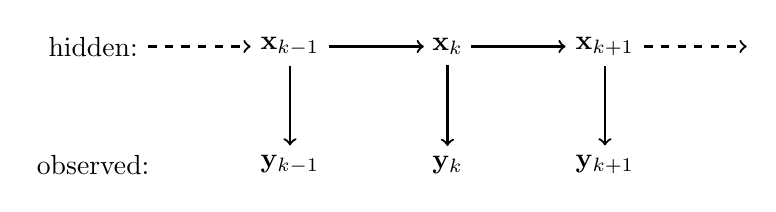
\begin{tikzpicture}
      \draw (0, 0) node {hidden:};
      \draw [->][dashed, thick] (0.7, 0) -- (2, 0);
      \draw (2.5, 0) node (x1) {$\mathbf{x}_{k-1}$};
      \draw [->][thick] (3, 0) -- (4.2, 0);
      \draw (4.5, 0) node (x2) {$\mathbf{x}_k$};
      \draw [->][thick] (4.8, 0) -- (6, 0);
      \draw (6.5, 0) node (x3) {$\mathbf{x}_{k+1}$};
      \draw [->][dashed, thick] (7, 0) -- (8.3, 0);

      \draw (0, -1.5) node {observed:};

      \draw (2.5, -1.5) node (y1) {$\mathbf{y}_{k-1}$};
      \draw [->][thick] (x1) -- (y1);
      \draw (4.5, -1.5) node (y2) {$\mathbf{y}_k$};
      \draw [->][thick] (x2) -- (y2);
      \draw (6.5, -1.5) node (y3) {$\mathbf{y}_{k+1}$};
      \draw [->][thick] (x3) -- (y3);
    \end{tikzpicture}
 \caption{A sequence of  hidden states $\mathbf{x}_k$ is indirectly
 observed through noisy measurements. Drawing recreated from \citep{sarkka2013bayesian}.}
    \label{fig:inversion}
\end{figure}

% TODO: reproduce figure of hidden variables and observations
% in Tikz side by side
% with  simple signal example  and measurement

We want to estimate the hidden states from the observed
measurements. Solving this problem in a Bayesian
sense means we 
need to compute the joint posterior distribution of all
states given all the measurements, for this we can simply
use Bayes' rule.
This yields a batch solution to the statistical estimation problem
resulting in the equation
\begin{equation}
  \label{eq:bayes}
  p(\mathbf{x}_{0:T} | y_{1:T})
  = \frac{p(y_{1:T} | \mathbf{x}_{0:T}) p(\mathbf{x}_{0:T})}
  {p(y_{1:T})}
\end{equation}
where $p(\mathbf{x}_{0:T})$ is the prior distribution defined by the dynamic
model, $p(y_{1:T} | \mathbf{x}_{0:T})$ is the likelihood model for the
measurements and $p(y_{1:T})$ is the normalization constant defined as
$$ p(y_{1:T}) = \int p(y_{1:T} | \mathbf{x}_{0:T})
p(\mathbf{x}_{0:T}) d \mathbf{x}_{0:T}.$$
This formulation is unfit for dynamic estimation tasks where
we receive measurements one at a time, since
at each time step we would have to
recompute the full posterior distribution. As the number of
time steps increases, also the dimensionality of the full posterior
would increase making computations intractable.
If we instead only compute selected marginal distributions we can
make computation feasible again. For this we need to restrict
our dynamic models to probabilistic Markov sequences, with a
transition probability distribution $p(\mathbf{x}_k | \mathbf{x}_{k-1})$.

In \textit{Bayesian filtering and smoothing} the following marginal
distributions are considered

\begin{itemize}
\item \textbf{Filtering distributions} computed by the
  Bayesian filter are the marginal distributions of the
  current state $\mathbf{x}_k$ given the current and previous measurements
  $y_{1:k} = \{y_1,...,y_k\}$
  $$ p(\mathbf{x}_k | y_{1:k}), \quad k = 1,...,T.$$
\item \textbf{Prediction distributions} which can be computed with
  the prediction step of the Bayesian filter are the marginal
  distributions of the future state $\mathbf{x}_{k+n}$, with $n$ steps
  after the current time step
  $$ p(\mathbf{x}_{k+n} | y_{1:k}), \quad k = 1,...,T \;\;\; n = 1,2,...$$
\item \textbf{Smoothing distributions} computed by the Bayesian smoother
  are the marginal distributions of the state $\mathbf{x}_k$ given
  a certain interval $y_{1:T} = \{y_1,...,y_T\}$ of measurements with
  $T > k$
  $$ p(\mathbf{x}_k | y_{1:T}), \quad k = 1,...,T$$
\end{itemize}

We will further discuss the filtering distribution,
as we use it for our surrogate model estimation problem.

For the filtering distribution we can formulate the recursive Bayesian
solution to the statistical inversion problem as follows:
\begin{enumerate}
\item The distribution of measurements is modeled by the likelihood
  function $p(y_k | \mathbf{x}_k)$ and the measurements are assumed
  to be conditionally independent
\item In the beginning at time step 0 all information about $\mathbf{x}$
  is contained in the prior distribution $p(\mathbf{x}_0)$
\item The measurements are assumed to be obtained one at a time,
  first $y_1$ then $y_2$ and so on. The key idea is to use the posterior
  distribution from the previous time step as the current prior
  distribution
  \begin{align*}
    p(\mathbf{x}_1 | y_{1}) &= \frac{1}{Z_1} p(y_1 | \mathbf{x}_1) p(\mathbf{x}_0) \\
    p(\mathbf{x}_2 | y_{1:2}) &= \frac{1}{Z_2} p(y_2 | \mathbf{x}_2) p(\mathbf{x}_1 | y_1) \\
                            &\vdots \\
    p(\mathbf{x}_k | y_{1:k}) &= \frac{1}{Z_k} p(y_k | \mathbf{x}_k)
                                p(\mathbf{x}_k | y_{1:k-1}) \\
                            &\vdots \\
    p(\mathbf{x}_T | y_{1:T}) &= \frac{1}{Z_T} p(y_T | \mathbf{x}_T) p(\mathbf{x}_{T-1} | y_{1:T-1})
  \end{align*}
  With the normalization term $Z_k = \int p(y_k | \mathbf{x}_k)
  p(\mathbf{x}_k | y_{1:k-1})
  d \mathbf{x}_k$. 
\end{enumerate}

This recursive formulation of Bayesian estimation has several useful
properties. First of all this can be considered as the
\textit{online learning} solution to the Bayesian learning problem.
As each step in the recursive estimation is a full Bayesian update step,
\textit{batch} Bayesian inference is a special case of recursive Bayesian
inference. Due to the sequential nature of the estimation we can model
what happens to the unknown quantity $\mathbf{x}$. This turns out
to be the basis of filtering theory, where time behavior is modeled
by assuming the quantity to be a time-dependent stochastic process
$\mathbf{x}(t)$.

\subsection{Least Squares}
To ease the application of Bayesian filtering to our specific problem
at a later stage we will now discuss a simple regression problem.
First we are going to derive the least squares solution, as
we use a least squares (LS) approach for comparison in our experiments.

We consider a simple linear regression problem,
\begin{equation}
  \label{regression_problem}
  y_k = x_1 + x_2 r_k + \epsilon_k
\end{equation}
where we assume that the measurement noise is zero mean Gaussian with
a given variance $\epsilon_k \sim \mathcal{N}(0, \sigma^2)$ and that the
prior distribution of the
parameters $\mathbf{x} = (x_{1} \; x_{2})^T$ is
Gaussian with known mean and covariance
$\mathbf{x} \sim \mathcal{N}(\mathbf{m}_0, \mathbf{P}_0)$. Note that
in this section the parameters $\mathbf{x}$ are assumed to stay constant.
We now want to estimate
the parameters $\mathbf{x}$ from a set of measurement
data $\mathcal{D} = \{(t_1, y_1),...,(t_T, y_T)\}$.

In compact in probabilistic notation the linear regression model
can be written as
\begin{equation}
  \label{regression_model_1}
  \begin{aligned}
    p(y_k | \mathbf{x}) &= \mathcal{N}(y_k | \mathbf{H}_k \mathbf{x}, \sigma^2) \\
    p(\mathbf{x}) &= \mathcal{N}(\mathbf{x} | \text{m}_0, \text{P}_0)
  \end{aligned}
\end{equation}
Here $\mathbf{H}_k = (1 \;t_k)$ is the design matrix and
contains the regressors and $\mathcal{N}(\cdot)$ denotes
the Gaussian probability density
function (see \Cref{gauss_pdf}). The row vector $\mathbf{H}_k$ is denoted
in matrix notation, to avoid using different notation for scalar
and vector measurements.
The batch solution can then be easily obtained by application of Bayes'rule
$$ p(\mathbf{x} | y_{1:T})
\propto p(\mathbf{x}) \prod^T_{k=1} p (y_k | \mathbf{x}) $$
$$ = \mathcal{N}(\mathbf{x} | m_0, P_0)
\prod^T_{k=1} \mathcal{N}(y_k | \textbf{H}_k \mathbf{x}, \sigma^2) $$

Because the prior and likelihood are Gaussian, the \textit{posterior distribution}
in turn is also Gaussian and denoted by
$$ p(\mathbf{x} | y_{1:T}) = \mathcal{N}(\mathbf{x} | m_t, P_t). $$

By completing the quadratic form in the exponent
we get the equations (\ref{LS}) for the mean and covariance
of the posterior distribution.
%- TODO: Do calculation in Appendix, (use canonical form)

\begin{equation}
  \label{LS}
  \begin{aligned}
    \mathbf{m}_T &= \left[ \mathbf{P}^{-1}_0 + \frac{1}{\sigma^2} \mathbf{H}^T \mathbf{H}
                   \right]^{-1} \left[\frac{1}{\sigma^2} \mathbf{H}^T \mathbf{y} +
                   \mathbf{P}^{-1}_0 \mathbf{m}_0 \right] \\
    \mathbf{P}_T &= \left[\mathbf{P}_0^{-1} + \frac{1}{\sigma^2} \mathbf{H}^T \mathbf{H}
                 \right]^{-1}
  \end{aligned}
\end{equation}
where $\mathbf{H}_k = (1 \;t_k)$ and
$$ \mathbf{H} =
\begin{pmatrix} \mathbf{H}_1 \\ \vdots \\ \mathbf{H}_T \end{pmatrix}
= \begin{pmatrix}
  1 \quad t_1 \\
  \vdots \quad \vdots \\
  1 \quad t_t
\end{pmatrix},
\quad \quad y = \begin{pmatrix} y_1 \\ \vdots \\ y_T \end{pmatrix}
$$

% TODO: write about realtionship to ordinary least squares and
% that we solve this with simply system of linear equations
% solving algorithm

\subsection{Kalman Filter} \label{KF}
%TODO: rework this section to use Kalman Filter instead of RLS
For the least squares solution, the parameters
$\mathbf{x} = (x_{1} \; x_{2})$ of
the regression model (\ref{regression_problem}) are assumed to stay constant.
Now, we assume the parameters are allowed to perform
a Gaussian random walk between measurements modeled by
\begin{align*}
  p(y_k | \mathbf{x}_k) &= \mathcal{N}(y_k | \mathbf{H}_k \mathbf{x}_k, \sigma^2) \\
  p(\mathbf{x}_k | \mathbf{x}_{k-1}) &= \mathcal{N}(\mathbf{x}_k |
                               \mathbf{x}_{k-1}, \mathbf{Q}) \\
  p(\mathbf{x}_0) &= \mathcal{N}(\mathbf{x}_0 | \mathbf{m}_0, \mathbf{P}_0)
\end{align*}
where $\mathbf{Q}$ is the covariance of the random walk. \\
We will now formulate the
linear regression model as a time-invariant model
by avoiding explicit covariates $t_k$.
This has the advantage that the model is not dependent on
the absolute time, but only on the relative positions of states
and measurements in time.
We denote the time difference between consecutive times as
$\Delta t_{k-1} = t_k - t_{k-1}$. The idea is that if
the underlying phenomenon (signal, state, parameter) $x_k$ was
exactly linear, the difference between adjacent time points could be
written exactly as
$$ x_k - x_{k-1} = \dot{x} \; \Delta t_{k-1} $$
where $\dot{x}$ is the derivative, which is constant in the linear case.
As this may not exactly be the case we also add some noise to the model
to get the following equations
\begin{align*}
  x_{1,k} &= x_{1,k-1} + \Delta t_{k-1} x_{2,k-1} + q_{1,k-1} \\
  x_{2,k} &= x_{2,k-1} + q_{2,k-1} \\
  y_k &= x_{1,k} + s_k
\end{align*}
where the signal is the first component of the state
($x_{1,k} = x_k$) and the derivative is the second
($x_{2,k} = \dot{x_k}$).
The noises are $s_k \sim \mathcal{N}(0, \sigma^2)$ and
$(q_{2,k-1}, q_{2,k-1}) \sim \mathcal{N}(0,\mathbf{Q})$.
Now, the linear regression model (\ref{regression_model_1}) can be written
in the form
\begin{align*}
  p(y_k | \mathbf{x}_k) &= \mathcal{N}(y_k | \mathbf{H}
                          \mathbf{x}_k, \sigma^2) \\
  p(\mathbf{x}_k | \mathbf{x}_{k-1}) &= \mathcal{N}(\mathbf{x}_k |
                                       \mathbf{A}_{k-1} \mathbf{x}_{k-1},
                                       \mathbf{Q})
\end{align*}
where
$$
\mathbf{A}_{k-1} =
\begin{pmatrix}
  1 & \Delta t_{k-1} \\
  0 & 1
\end{pmatrix}, \quad \quad \mathbf{H} = (1 \quad 0)
$$

In this formulation the model is a special case of generic linear Gaussian
models of the form, 
\begin{align*}
  p(y_k | \mathbf{x}_k) &= \mathcal{N}(y_k | \mathbf{H}_k \mathbf{x}_k,
                          \mathbf{R}_k) \\
  p(\mathbf{x}_k | \mathbf{x}_{k-1}) &= \mathcal{N}(\mathbf{x}_k
                                      | \mathbf{A}_{k-1} \mathbf{x}_{k-1},
                                      \mathbf{Q}_{k-1})
\end{align*}
for which the Kalman Filter \citep{Kalman:1960} is the optimal recursive solution
(for the full derivation see  \cref{KF_appendix}).

% \newpage
% $$~$$

The Kalman filter equations can be expressed as
prediction and update steps as follows:
\begin{itemize}
\item The prediction step
  \begin{equation}
    \label{KF_prediction}
    \begin{aligned}
      \mathbf{m}_k^- &= \mathbf{A}_{k-1} \mathbf{m}_{k-1} \\
      \mathbf{P}_k^- &= \mathbf{A}_{k-1} \mathbf{P}_{k-1} \mathbf{A}^T_{k-1}
      + \mathbf{Q}_{k-1}
    \end{aligned}
  \end{equation}

\item The update step
  \begin{equation}
    \label{KF_update}
    \begin{aligned}
      v_k &= y_k - \mathbf{H}_k \mathbf{m}_k^- \\
      \mathbf{S}_k &= \mathbf{H}_k \mathbf{P}_k^T \mathbf{H}^T_k +
      \mathbf{R}_k \\
      \mathbf{K}_k &= \mathbf{P}_k^- \mathbf{H}_k^T \mathbf{S}_k^{-1} \\
      \mathbf{m}_k &= \mathbf{m}_k^- + \mathbf{K}_k v_k \\
      \mathbf{P}_k &= \mathbf{P}_k^- - \mathbf{K}_k \mathbf{S}_k \mathbf{K}_k^T
    \end{aligned}
  \end{equation}
\end{itemize}

% TODO: For the full derivation see appendix (cite)

